\documentclass[a4paper, 12pt, dvipdfmx, uplatex]{jsreport}
% \usepackage[top=30truemm, bottom=30truemm, left=25truemm, right=25truemm]{geometry} % 余白設定
% \usepackage[dvipdfmx]{pdflscape}


\usepackage{url}
% \usepackage{moreverb}

\usepackage{listings,jvlisting} %ソースコード埋め込み
\lstset{
  basicstyle={\ttfamily},
  identifierstyle={\small},
  commentstyle={\smallitshape},
  keywordstyle={\small\bfseries},
  ndkeywordstyle={\small},
  stringstyle={\small\ttfamily},
  frame={tb},
  breaklines=true,
  columns=[l]{fullflexible},
  numbers=left,
  xrightmargin=0zw,
  xleftmargin=3zw,
  numberstyle={\scriptsize},
  stepnumber=1,
  numbersep=1zw,
  lineskip=-0.5ex
}
\makeatletter
\def\lst@lettertrue{\let\lst@ifletter\iffalse}
\makeatother
\renewcommand{\lstlistingname}{プログラム}

% ================ Quick Half Quad Text bgn =========================
\newcommand{\hqq}[1]{\ \mathtt{#1}\ }
\newcommand{\hqif}{\hqq{if}}
\newcommand{\hqthen}{\hqq{then}}
\newcommand{\hqelse}{\hqq{else}}
\newcommand{\hqwhile}{\hqq{while}}
\newcommand{\hqdo}{\hqq{do}}
\newcommand{\hqskip}{\hqq{skip}}

\newcommand{\hqql}[1]{\ \mathtt{#1}}
\newcommand{\hqlif}{\hqql{if}}
\newcommand{\hqlthen}{\hqql{then}}
\newcommand{\hqlelse}{\hqql{else}}
\newcommand{\hqlwhile}{\hqql{while}}
\newcommand{\hqldo}{\hqql{do}}
\newcommand{\hqlskip}{\hqql{skip}}

\newcommand{\hqqr}[1]{\mathtt{#1}\ }
\newcommand{\hqrif}{\hqqr{if}}
\newcommand{\hqrthen}{\hqqr{then}}
\newcommand{\hqrelse}{\hqqr{else}}
\newcommand{\hqrwhile}{\hqqr{while}}
\newcommand{\hqrdo}{\hqqr{do}}
\newcommand{\hqrskip}{\hqqr{skip}}

\newcommand{\nhqq}[1]{\mathtt{#1}}
\newcommand{\nhqskip}{\nhqq{skip}}
\newcommand{\x}{\nhqq{x}}
\newcommand{\y}{\nhqq{y}}
\newcommand{\z}{\nhqq{z}}
% ================ Quick Half Quad Text end =========================

%定理環境
\theoremstyle{definition}
\newtheorem{dfn}{定義}
\newtheorem{thm}{定理}
\newtheorem{lemma}{補題}

\usepackage[dvipdfmx]{graphicx} % グラフを入れるのに必要
\usepackage[dvipdfmx]{color} % グラフを入れるのに必要
\usepackage{fancyhdr} % ページ数指定に必要
\usepackage{lastpage} % 同上
\usepackage{multirow} % 表で縦複数行にまたがるセルを作るのに必要
\usepackage{amsmath} % 一部の数学記号や数学的表現をするために必要
\usepackage{autobreak}
\usepackage{amsfonts} % 同上
\usepackage{amssymb} % 同上
\usepackage{bm} % 太字に必要
\usepackage{siunitx} % SI単位系の斜体を直す
\usepackage{here}
\usepackage{wrapfig}
\usepackage{breqn} % dmath でいい感じに数式を折り返してくれる
% \usepackage{pdfpages} % pdf を挿入できる
% \usepackage{slashbox} % 表に斜め線を入れるやつ このtexファイルがあるディレクトリと同じところにslashbox.styを置くとかする必要がある。

\usepackage{breqn}
\usepackage{wrapfig}
\usepackage{physics}
\usepackage{mathrsfs}
\usepackage{mathtools}
\usepackage{bussproofs}

\usepackage{lscape}

% \newcommand{\unit}[1]{\mathrm{[#1]}} % 単位の括弧[]
\newcommand{\tup}[1]{\left\langle{#1}\right\rangle}

% % タイトルを明朝体で書く
% % \titleformat* は \titleformat を短く書く方法. 
\usepackage{titlesec}
% \titleformat*{\section}{\Large\bfseries}
% \titleformat*{\section}{\large\bfseries}
% \titleformat*{\subsection}{\large\bfseries}
% \titleformat*{\subsection}{\normalsize\bfseries}
% \titleformat*{\subsubsection}{\normalsize\bfseries}

% ページの右下にページ数を記載するスタイル
% \fancypagestyle{mypagestyle}{
%   \lhead{}
%   \rhead{}
%   \fancyfoot[C]{}
%   \fancyfoot[R]{p.\thepage/\pageref{LastPage}}
%   \renewcommand{\headrulewidth}{0.0pt}
% }

% ページスタイルを適用
% \pagestyle{mypagestyle}

% \maketitle コマンドをdocument内に入れることで, タイトルページが自動生成される
% \title{プログラミング言語特論 \quad 課題1}
% \author{1W192258-2 \quad 富家功一朗}

% \makeatletter
%   \renewcommand{\thesubsection}{\arabic{section}.\arabic{subsection}}
%   \@addtoreset{subsection}{section}
% \makeatother

% \renewcommand{\thesection}{\textbf{[\arabic{section}]}}
% \renewcommand{\thesubsection}{(\alph{subsection})}

% 式番号を章.式番 の形式にさせる
%  \makeatletter
%    \renewcommand{\theequation}{\arabic{section}.\arabic{equation}}
%    \@addtoreset{equation}{section}
%  \makeatother

% 表番号も
%  \makeatletter
%    \renewcommand{\thetable}{\arabic{section}.\arabic{table}}
%    \@addtoreset{table}{section}
%  \makeatother

% 図番号も
%  \makeatletter
%    \renewcommand{\thefigure}{\arabic{section}.\arabic{figure}}
%    \@addtoreset{figure}{section}
%  \makeatother

% ソースコード番号も
%  \makeatletter      
%       \AtBeginDocument{                       
%           \renewcommand*{\thelstlisting}{\arabic{section}.\arabic{lstlisting}}          
%           \@addtoreset{lstlisting}{section}                    
%       }            
%  \makeatother

% 参考文献の番号を 1) にする
% \makeatletter
%   \def\@biblabel#1{#1)}
% \makeatletter

% 図の入れ方
% \begin{figure}[H] % h...hereの意
%   \centering
%   \includegraphics[width=13cm]{kairo.png}
%   \caption{キャプション名\label{ラベル名}}
% \end{figure}

% 回り込む図
% \begin{wrapfigure}[13]{r}{5cm}
%   \centering
%   \includegraphics[width=5cm]{img/schematics.png}
%   \vspace*{-\intextsep}
%   \caption{システムの模式図\label{schematics}}
% \end{wrapfigure}

% 表の入れ方
% \begin{table}[H]
%   \centering
%   \caption{キャプション名\label{ラベル名}}
%   \begin{tabular}{c|c|c|c} \hline \hline
%     抵抗名 &$\zeta$ &$\psi$ & $g :\ \mathrm{dB}$ \\\hline
%     R1&$0.0500$ &$ 0.997 $ & $20.0$\\\hline
%     R3 & $0.500$ &$0.707$ & $2.32$ \\\hline
%   \end{tabular}
% \end{table}

% ソースコードの埋め込み方
% \begin{lstlisting}[caption=name,label=number]
% \end{lstlisting}

% pdf 挿入の仕方
% \includepdf[pages=-]{pdfs/reviews.pdf}
% \includepdf[pages=3]{pdfs/FrontCovers.pdf}
% \includepdf[pages=2-]{pdfs/report1.pdf}

% prooftree
% \begin{prooftree}
%   \AxiomC{}
%   \RightLabel{$\overrightarrow{\mathtt{var}}$}
%   \UnaryInfC{$\tup{x, s}\to \tup{1, s}$}
%   \RightLabel{$\overrightarrow{\mathtt{op1}}$}
%   \UnaryInfC{$\tup{x\leq y, s}\to \tup{1\leq y, s}$}
%   \RightLabel{$\overrightarrow{\mathtt{if1}}$}
%   \UnaryInfC{$\tup{\hqrif x \leq y \hqthen C_1 \hqelse \nhqskip, s}\to \tup{\hqrif 1 \leq y \hqthen C_1 \hqelse \nhqskip, s}$}
%   \RightLabel{$\overrightarrow{\mathtt{seq1}}$}
%   \UnaryInfC{$\tup{(\hqrif x \leq y \hqthen C_1 \hqelse \nhqskip );(z \coloneqq 3; C_2), s}\to \tup{(\hqrif 1 \leq y \hqthen C_1 \hqelse \nhqskip );(z \coloneqq3; C_2), s}$}
% \end{prooftree}

\setcounter{tocdepth}{3}

\title{ReDoS脆弱な正規表現の修正}
\author{情報理工学科 寺内研究室所属 富家功一朗}
\date{2023年1月31日}

\begin{document}
\chapter{準備}
\section{正規表現}
正規表現とは言語(文字列の集合)を一つの文字列で表現する方法である.正規表現は文字列のパターンマッチングなどに使われ,その実用性の高さから多くのプログラミング言語で扱うことができる.実世界のプログラミング言語で使用されるような正規表現の中には,正規言語(ある正規表現にマッチする文字列全体の集合)以上の表現力を持つものもある(後方参照の機能を提供している正規表現など)が,本論文では次に示すように純粋な正規表現を対象とする.

\subsection{正規表現の構文}
本論文で扱う正規表現の構文を以下に示す.
\begin{figure}[h]
  \centering
  \setlength{\fboxrule}{0.5pt}
  \fbox{
      $\begin{array}{llcl}
          \text{正規表現}&r&\coloneqq&\ \ \: \varepsilon\\
              &&&\mid \ c\\
              &&&\mid \ r_1 \mid r_2\\
              &&&\mid \ r_1r_2\\
              &&&\mid \ r^*\\
      \end{array}$
  }
  \caption{正規表現の構文}
  \label{fig:syntax-regex}
\end{figure}

$\varepsilon$は空列を表す定数,$c$は任意の1文字(本論文ではASCIIコードを想定している)を表す定数,$r,r_1,r_2$は正規表現を表す変数とする.$r_1 \mid r_2$は選択,すなわち$r_1$に含まれる文字列の集合と$r_2$に含まれる文字列の集合の和集合を表す.$r_1r_2$は連接,すなわち$r_1$に含まれる文字列に$r_2$に含まれる文字列をつなげてできる文字列の集合を表す.$r^*$はクリーネ閉包,すなわち$r$に含まれる文字列を0個以上つなげてできる文字列の集合を表す.

また,本論文では先の正規表現で表現可能ないくつかの拡張機能を搭載している.以下にどのような拡張を搭載したか述べる.
\begin{itemize}
  \item $.$ \quad 任意の1文字にマッチすることを表す.
  \item $[a_ia_{i+1}\ldots a_j]$ \quad $a_i,a_{i+1},\ldots ,a_j$のうちのどれか1文字にマッチすることを表す.特に,$[a_i$-$a_j]$は文字コード上で$i$から$j$番目にある文字のうちどれか1文字にマッチすることを表す.
  \item $[$^$a_ia_{i+1}\ldots a_j]$ \quad $a_i,a_{i+1},\ldots ,a_j$以外のどれか1文字にマッチすることを表す.
  \item $r?$ \quad 正規表現$r$に属する文字列が0回または1回出現することを表す.
\end{itemize}



\subsection{正規表現を用いた文字列のパターンマッチング例}
正規表現を用いた文字列のパターンマッチング例を見る.$a\mid b$という正規表現には$a,b$といった文字列がマッチする.$ab$という正規表現には$ab$といった文字列がマッチする.$a^*$という正規表現には$\varepsilon,a,aa,aaa,\ldots$といった文字列がマッチする.最後に,$(a|bc)^*$という正規表現には$\varepsilon,a,bc,aa,abc,bca,bcbc,\ldots$といった文字列がマッチする.

また,本論文で扱うような正規表現においてパターンマッチングに成功した(正規表現に受理されるとも言う)文字列集合を正規言語と呼ぶ.そして,ある正規表現$\mathcal{A}$に受理される言語のことを$\mathcal{L(A)}$と書くことにする.


\section{NFA}
NFA(Nondeterministic Finite Automaton)は有限オートマトンの一種で,ある状態から入力を受け取ったとき,次の状態への遷移が一意に決まらないことがあるものである.正規表現はそれと等価なNFAへと変換することが可能であるので,今後は正規表現のままではなくそれと等価なNFAを用いることにより議論を進めることがある.

% 後で書く
\subsection{NFAの定義}
先行研究で紹介されていたNFAの定義を以下に示す.
\begin{dfn}[($\varepsilon$遷移なし)NFA]
  NFA $\mathcal{A}$は5つの組$(Q,\Sigma,\Delta,q_0,F)$からなる.$Q$は状態の有限集合,$\Sigma$はアルファベット(文字)の有限集合,$\Delta :Q\times \Sigma \rightarrow 2^Q$は遷移関数である.$q_0 \in Q$を初期状態,$F \subseteq Q$を受理状態の集合とする.また,もし$q'\in \Delta (q,l)$なら$(q,l,q')$をラベルを経由した遷移と呼ぶこととする.
\end{dfn}

また,関連してパスという用語の定義も行う.

\begin{dfn}[($\varepsilon$遷移なしNFAにおける)パス]
  NFA $\mathcal{A}=(Q,\Sigma,\Delta,q_0,F)$のパス$\pi$を遷移列,すなわち$(q_1,l_1,q_2),\ldots,(q_{m-1},l_{m-1},q_{m})$とする.ただし,$q_i \in Q$,$l_i \in \Sigma$,$q_{i+1} \in \Delta(q_i,l_i)$である.つまり,$\pi$は$q_i$から始まって$q_m$で終わるパスを表す.また,labels$(\pi)$はラベル列,$(l_1,\ldots ,l_{m-1})$を意味するものとする.
\end{dfn}


このNFAの定義は一般的ではない.$\Sigma$に空列$\varepsilon$を加えた$\Sigma \cup \qty{\varepsilon}$をアルファベット集合として5つ組$(Q,\Sigma \cup \qty{\varepsilon},\Delta,q_0,F)$をNFAの定義とすることが多い.すなわち,

\begin{dfn}[NFA]
  NFA $\mathcal{A}$は5つの組$(Q,\Sigma \cup \qty{\varepsilon},\Delta,q_0,F)$からなる.$Q$は状態の有限集合,$\Sigma$はアルファベット(文字)の有限集合,$\varepsilon$は空列,$\Delta :Q\times \Sigma \rightarrow 2^Q$は遷移関数である.$q_0 \in Q$を初期状態,$F \subseteq Q$を受理状態の集合とする.また,もし$q'\in \Delta (q,l)$なら$(q,l,q')$をラベルを経由した遷移と呼ぶこととする.
\end{dfn}

また,パスも以下のように書き換える.
\begin{dfn}[パス]
  NFA $\mathcal{A}=((Q,\Sigma \cup \qty{\varepsilon},\Delta,q_0,F))$のパス$\pi$を遷移列,すなわち$(q_1,l_1,q_2),\ldots,(q_{m-1},l_{m-1},q_{m})$とする.ただし,$q_i \in Q$,$l_i \in \Sigma \cup \qty{\varepsilon}$,$q_{i+1} \in \Delta(q_i,l_i)$である.つまり,$\pi$は$q_i$から始まって$q_m$で終わるパスを表す.また,labels$(\pi)$はラベル列,$(l_1,\ldots ,l_{m-1})$を意味するものとする.
\end{dfn}


今後はただNFAとだけ記載した場合,$\varepsilon$遷移ありのNFAを指す.

NFAに文字列を入力したとき,初期状態$q_0$から始まって一つずつ文字を読み取って遷移していき,ちょうど受理状態に到達するとき,その文字列はNFAに受理されるという.受理状態以外の状態で読み取りが終了した場合,その文字列はNFAに拒絶されるという.NFAに受理される文字列全体の集合をNFAの受理する言語という.



\subsection{$\varepsilon$遷移なしNFAの例}
($\varepsilon$遷移なし)NFA $\mathcal{A}_1$を$(\qty{q,q'},\qty{a,b},\Delta,q,\qty{q'})$とする.なお,遷移関数$\Delta$は以下のような状態遷移表で表されるものとする.表の縦軸が状態,横軸がアルファベットを表す.ある状態とあるアルファベットが交差するセルは,ある状態からあるアルファベットを読んで遷移する状態の集合を表している.例えば,状態$q$からアルファベット$a$を読んで遷移する状態の集合は$\qty{q,q'}$である.

\begin{table}[H]
  \centering
  \caption{遷移関数$\Delta$\label{delta}}
  \begin{tabular}{c|c|c} \hline \hline
       & $a$  &$b$ \\\hline
    $q$  & $\qty{q,q'}$ &$\qty{}$ \\\hline
    $q'$ & $\qty{}$  &$\qty{q,q'}$ \\\hline
  \end{tabular}
\end{table}

NFA $\mathcal{A}_1$をグラフにすると以下のようになる.
\begin{figure}[H] % h...hereの意
  \centering
  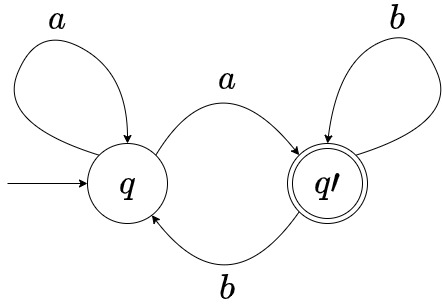
\includegraphics[width=0.5\linewidth]{/home/thelema/KoichiroTomiie_thesis_2022/figures/nfa.jpg}
  \caption{NFA $\mathcal{A}_1$\label{nfa_example}}
\end{figure}

このNFAが受理する言語は$\qty{a,aa,ab,aaa,aab,aba,abb,\ldots}$である.これは正規表現$a(a|b)^*$に対応する.

% \subsection{DFA}

\section{正規表現の等価性判定}
2つの正規表現が等価であるとはどういうことか,また等価性判定がどのようなアルゴリズムで行われているのかを述べる.

\subsection{正規表現の等価性}
ある2つの正規表現$\mc{A},\mc{B}$が存在し,それらの正規表現にマッチする文字列の集合(つまり正規言語)が等しいとき,すなわち$\mc{L(A)}=\mc{L(B)}$であるとき,$\mc{A},\mc{B}$は意味的に等価であるという.以下に例を挙げる.

2つの正規表現が構文的に等しい場合,例えば$\mc{A}=x^*,\mc{B}=x^*$としたとき,$\mc{L}(x^*)=\qty{\varepsilon,x,xx,xxx,\ldots}$よりこれらは意味的にも等しい.

2つの正規表現が構文的に等しくなく,意味的に等しい場合について考える.例えば$\mc{A}=x^*,\mc{B}=x^*x^*$としたとき,これらは構文的に等しくないが,$\mc{L}(x^*)=\mc{L}(x^*x^*)=\qty{\varepsilon,x,xx,xxx,\ldots}$より意味的には等しい.

\subsection{正規表現の等価性判定アルゴリズム}\label{eq_check}
正規表現の等価性判定を行う方法はいくつか知られている.

例えば,有名なアルゴリズムとして次のようなものがある.まず2つの正規表現をNFA化する.次に2つのNFAをDFA(Deterministic Finite Automaton,ある状態からの遷移先が一意に定まった有限オートマトン)化する.さらに2つのDFAを最小化(不要な状態の削減)する.最小化した際に得られるDFAは一意に定まることが知られている.この事実を利用し,2つの最小DFAが一致するかどうかを確認することで等価性判定を行うことができる.上記のようなアルゴリズムは\cite{hopcroft}で紹介されている.

また,他にも正規表現の微分(\cite{regex_de1},\cite{regex_de2})を利用した等価性判定アルゴリズム\cite{regex_eq_de}がある.

しかし,本研究では先の2つのアルゴリズムではなく,次のようなアルゴリズムを用いることにする(このアルゴリズムも有名で\cite{sipser}で紹介されている).

\begin{enumerate}
  \item 2つの正規表現$\mc{A},\mc{B}$をNFA化し,さらにDFA化し,それらを$\mc{A}_{DFA},\mc{B}_{DFA}$とする.
  \item $\mc{A}_{DFA}$と$\mc{B}_{DFA}$の否定を取ったDFA($\overline{\mc{B}_{DFA}}$と表記する)との積を取り,これを$\mc{A}_{DFA}\cap\overline{\mc{B}_{DFA}}$と表記する.また,同様に$\overline{\mc{A}_{DFA}}\cap\mc{B}_{DFA}$も構成する.なお,正規言語は積集合演算,補集合演算について閉じているので,これらもまたDFAである.
  \item $\mc{L}(\mc{A}_{DFA}\cap\overline{\mc{B}_{DFA}})=\varnothing$かつ$\mc{L}(\overline{\mc{A}_{DFA}}\cap\mc{B}_{DFA})=\varnothing$なら2つの正規表現$\mc{A},\mc{B}$は等価,そうでないなら等価ではない.
\end{enumerate}

ここでDFAの積,否定を取る工程が発生しているが,具体的な構成方法は\cite{sipser}を参照されたい.また,正規言語の空性判定についても\cite{sipser}を参照されたい.

このアルゴリズムのメリットとして2つの正規表現が等価でないことを示す反例を探しやすいということが挙げられる.後に提案する手法ではこの反例を利用する.



% \bibliography{main}
% \bibliographystyle{junsrt}


\end{document}